\label{sec:af_squarkgluino}
The most stringent limits on sparticles generally come from inclusive
searches for strongly produced light squarks and gluinos, in particular into
all hadronic final states. In ATLAS, these searches are performed
within the inclusive squark and gluino SUSY sub-group, composed of
approximately 140 members and presently split into eight paper streams
based on the number of jets and lepton flavors in the final state.
UTA has been involved in these searches since beginning of Run 1,
twice convening this subgroup (UTA postdocs David Cote and Heelan),
and most recently supervising several public papers and conference
notes for ICHEP
2016~\cite{Aad:2016jxj,Aaboud:2016zdn,Aad:2016qqk,ATLAS-CONF-2015-082,Aad:2016tuk,Aad:2016eki,Aaboud:2016zpr,ATLASCollaboration:2016wlb,ATLAS-CONF-2016-078,ATLAS-CONF-2016-054,ATLAS-CONF-2016-037,ATLAS-CONF-2016-052,ATLAS-CONF-2016-066,ATLAS-CONF-2016-095}. Heelan
also directly contributed to the search for SUSY in all hadronic
states, which is a flagship SUSY search.

Between 2010-15, Farbin's ECRP grant supported introduction of novel
``event view'' techniques to search for SUSY, with the Razor
reconstruction technique~\cite{Rogan:2010kb} in 2011\cite{Aad:2012naa}
and 2012 ~\cite{Aad:2015iea}. The most recent iteration of this line
of searches, based on an extension called the Recursive Jigsaw
Reconstruction (RJR), was fully integrated into the mainstream Run 2
search performed for ICHEP2016~\cite{ATLAS-CONF-2016-078} and was the
final topic of Bullock's now completed PhD
thesis~\cite{BullockThesis}. The RJR groups all final state objects
into hemispheres based on assumptions (or views) about how the decay
is proceeding, providing an uncorrelated basis of observables
consisting of energy scales (masses, transverse quantities) and
scaleless variables (like angles between hemispheres and ratios of
energy scale variables). RJR-based selections generally only partially
overlap with standard selections (i.e. based on missing transverse
momentum, $H_\mathrm{T}$, etc.), for example bringing in an observed
50\% additional events in the all hadronic final state and thereby
extending both the phase space and the statistical reach of such
searches (if properly combined).

%Figure~\ref{fig:ICHEPLimits} shows that in general across simplified
%model planes representing these type of models the new RJR method had
%an expected sensitivity similar to that of the standard detector-based
%variables.

%Figure~\ref{fig:RJRTrees}
%the conference note and
%~\cite{Jackson:2016mfb}
%An example of the views used in the latest analysis presented at
%ICHEP2016 are shown in Figure~\ref{fig:RJRTrees}. 
%For ICHEP2016,  these views enabled defining signal regions

\begin{figure}[tb]
\centering
\subfigure{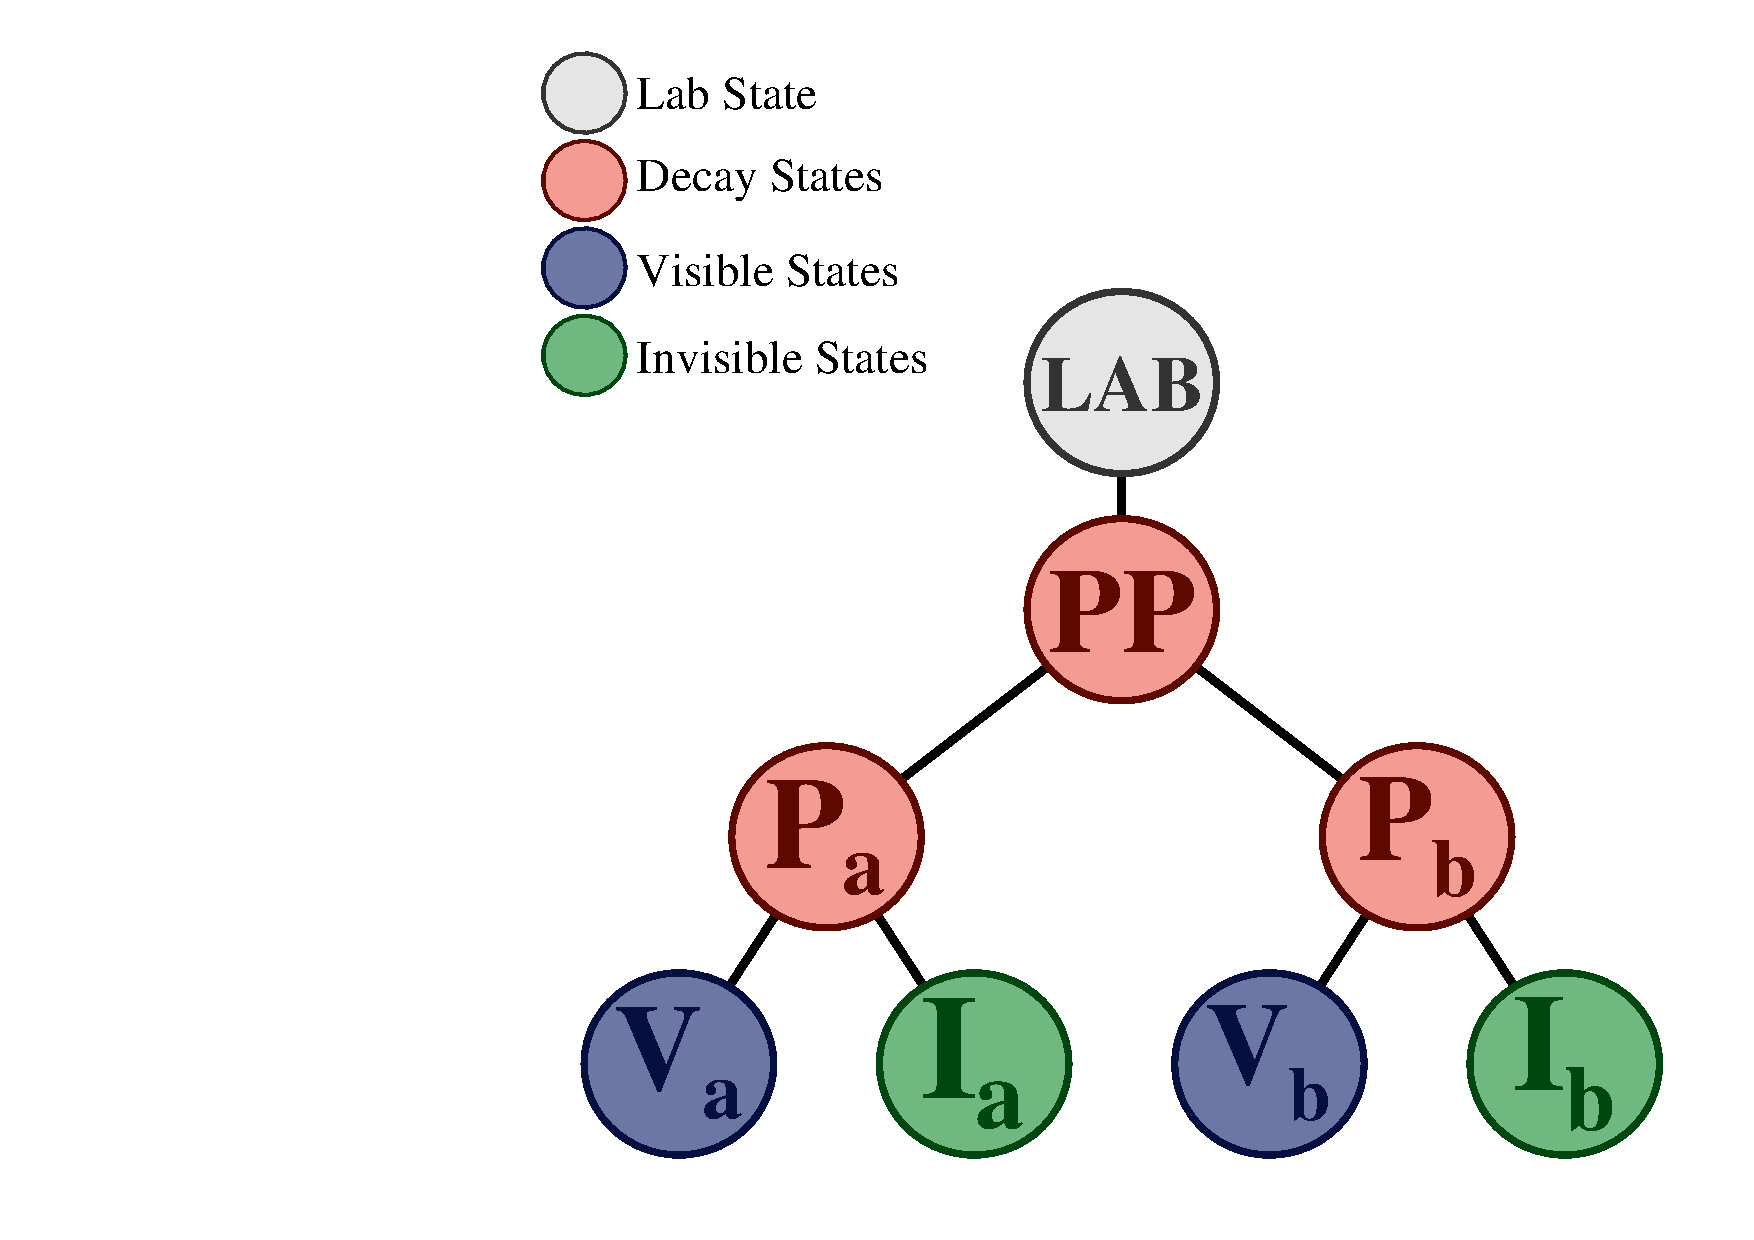
\includegraphics[width=0.30\textwidth]{Farbin/Figures/RJRtree_DiSparticle.pdf}}
\subfigure{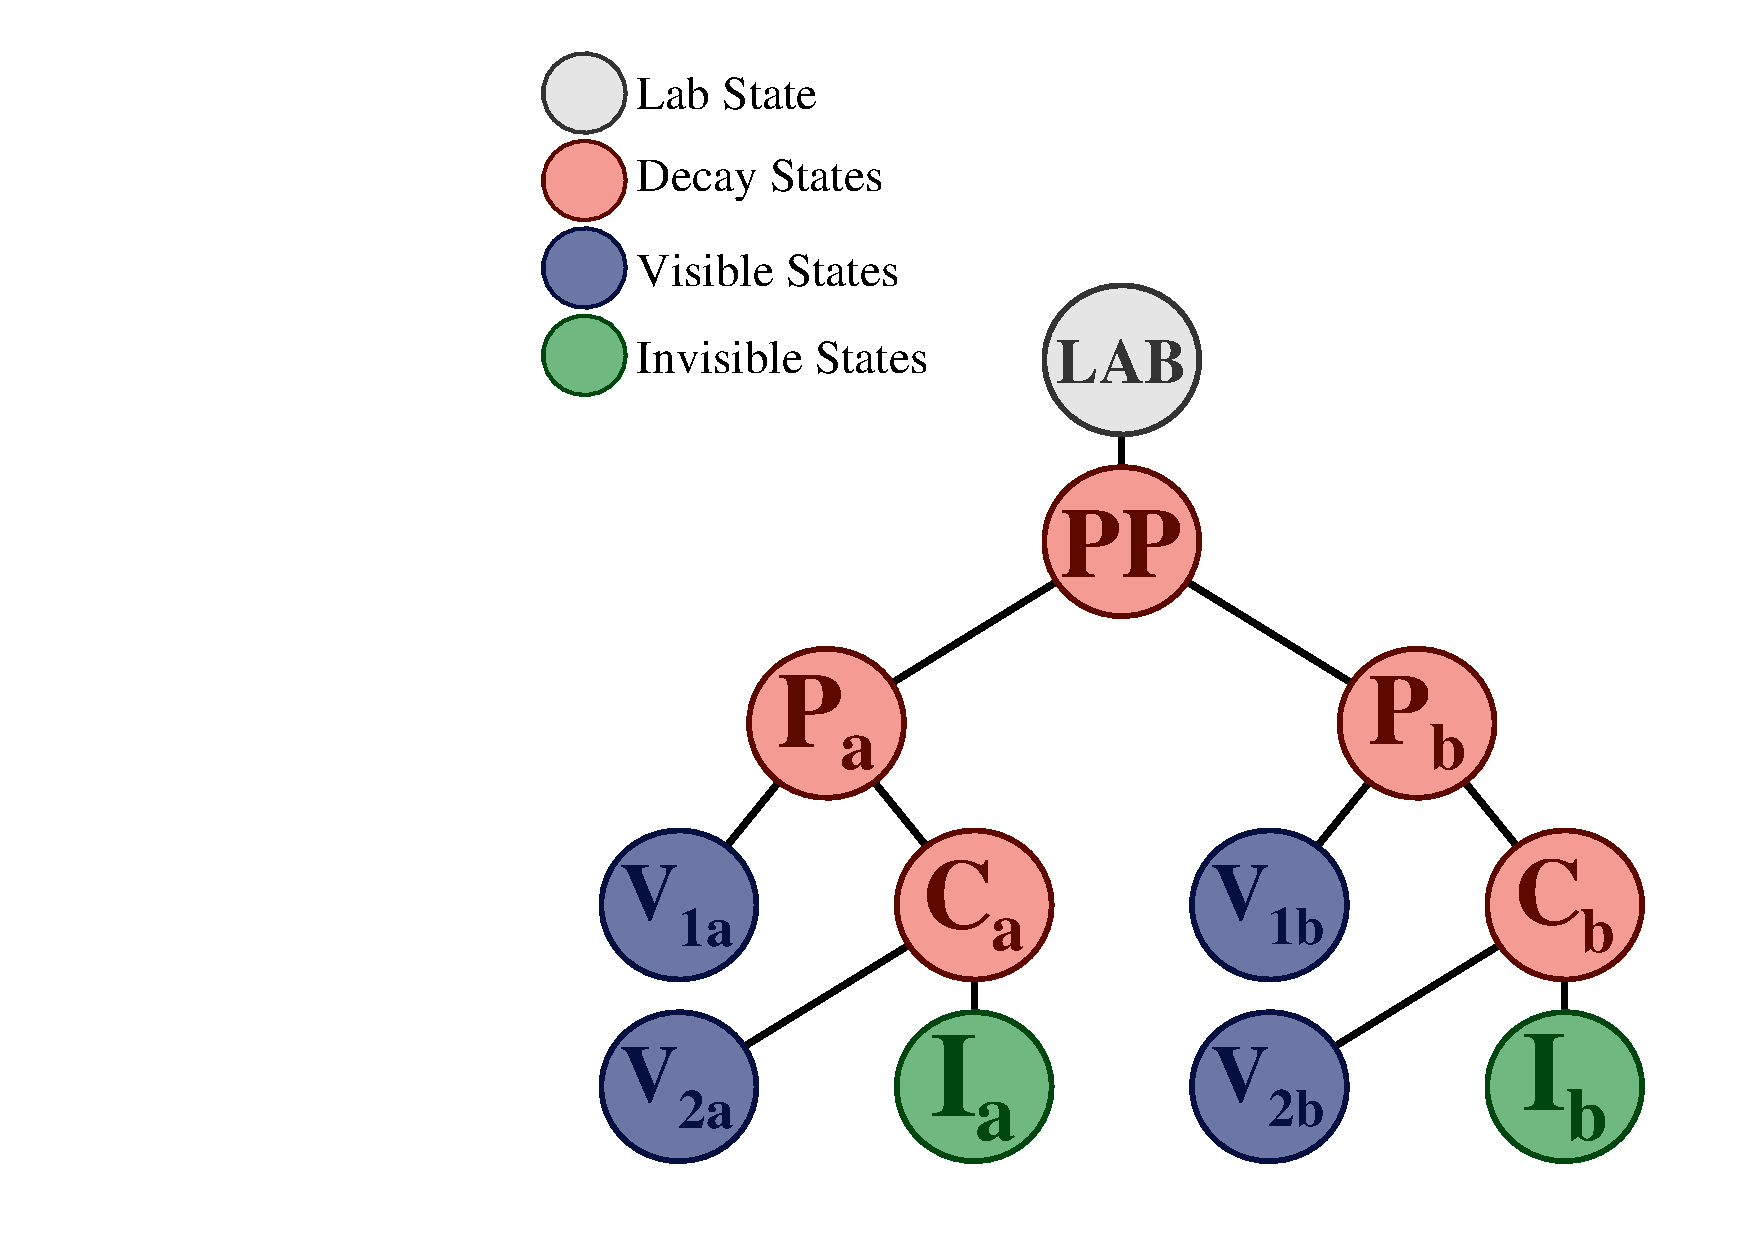
\includegraphics[width=0.30\textwidth]{Farbin/Figures/RJRtree_DiGluino.pdf}}
\subfigure{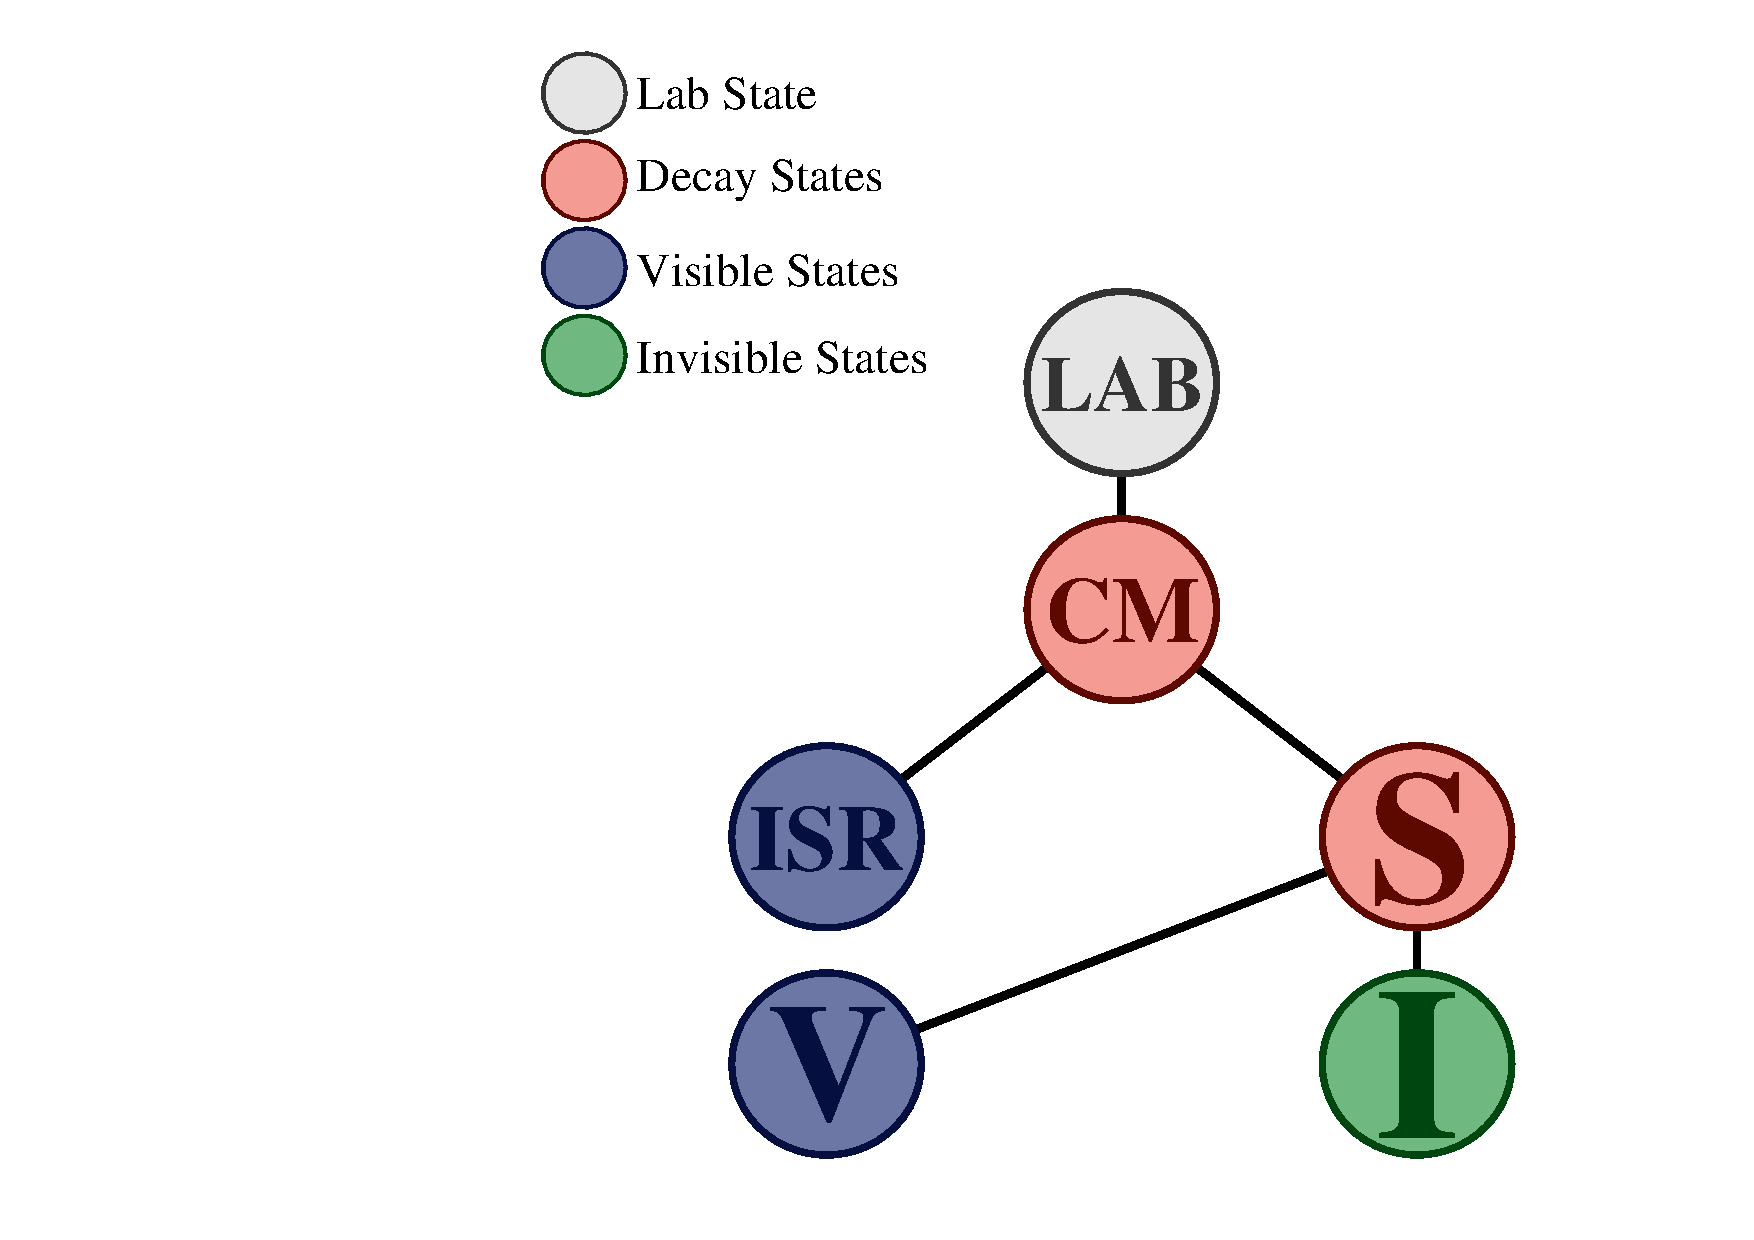
\includegraphics[width=0.30\textwidth]{Farbin/Figures/RJRtree_Compressed.pdf}}
\caption{\label{fig:RJRTrees} 
Recursive Jigsaw Reconstruction event views for three scenarios: (a)
Two sparticles ($P_{a}$ and $P_{b}$) are pair-produced with each
decaying to one or more visible particles ($V_{a}$ and $V_{b}$) which
are reconstructed in the detector, and two systems of invisible
particles ($I_{a}$ and $I_{b}$) whose four-momenta are only partially
constrained. (b) An additional level of decays can be added when
requiring more than two visible objects. (c) Strong sparticle
production with an ISR decay tree for use with small mass-splitting
spectra, where a single sparticle system $S$ decays to a set of
visible momenta $V$ and invisible momentum $I$, and recoils off of a
jet radiation system ISR.  }
\end{figure}

The RJR views used for ICHEP2016, shown in figure~\ref{fig:RJRTrees},
were designed to search for SUSY produced by squark or gluino pair
production and direct decay to final states containing jets and the
lightest supersymmetric particle. While this RJR technique had a
standalone expected sensitivity similar to that of the standard
technique, RJR extended sensitivity by also targeting difficult
phase-space regions with views of Compressed Spectra (CSS) scenarios
where all final state objects are assumed to recoil off an ISR
jet~\cite{Jackson:2016mfb}. In CSS, small mass splittings between the
heavier produced sparticle and lightest SUSY particle (LSP) lead to
soft final state objects and missing transverse momentum that fail
traditional scale-depended background suppression selections.

As evident in the ICHEP2016 conference
note~\cite{ATLAS-CONF-2016-078}, the RJR ISR event view extended the
squark and gluino exclusion limits with respect to the standard
effective mass analysis for the squark-squark and gluino-pair
production cases by as much as 50\% and 100\%, respectively, reducing
mass differences sensitivity by 50~GeV to $\Delta m(\tilde{q} -
\chi_1^0) = 100~\mathrm{GeV}$ at $m_{\tilde{q}} = 700~\mathrm{GeV}$  and 
$\Delta m(\tilde{g} -\chi_1^0) = 50~\mathrm{GeV}$ at $m_{\tilde{g}} =
925~\mathrm{GeV}$. For Run 2, Farbin's student Bullock helped Rogan
(Harvard) and Jackson (Adelaide) implement and commission a
Razor-based high-level trigger that uses only scale-less quantities
and therefore enhances CSS trigger efficiencies. This trigger is not
yet used in Run 2 searches because the prescale threshold for the
missing energy triggers are still below the expectations and the
corresponding optimization of the running Razor trigger.



%% \begin{figure}[tb]
%% \centering
%% \subfigure{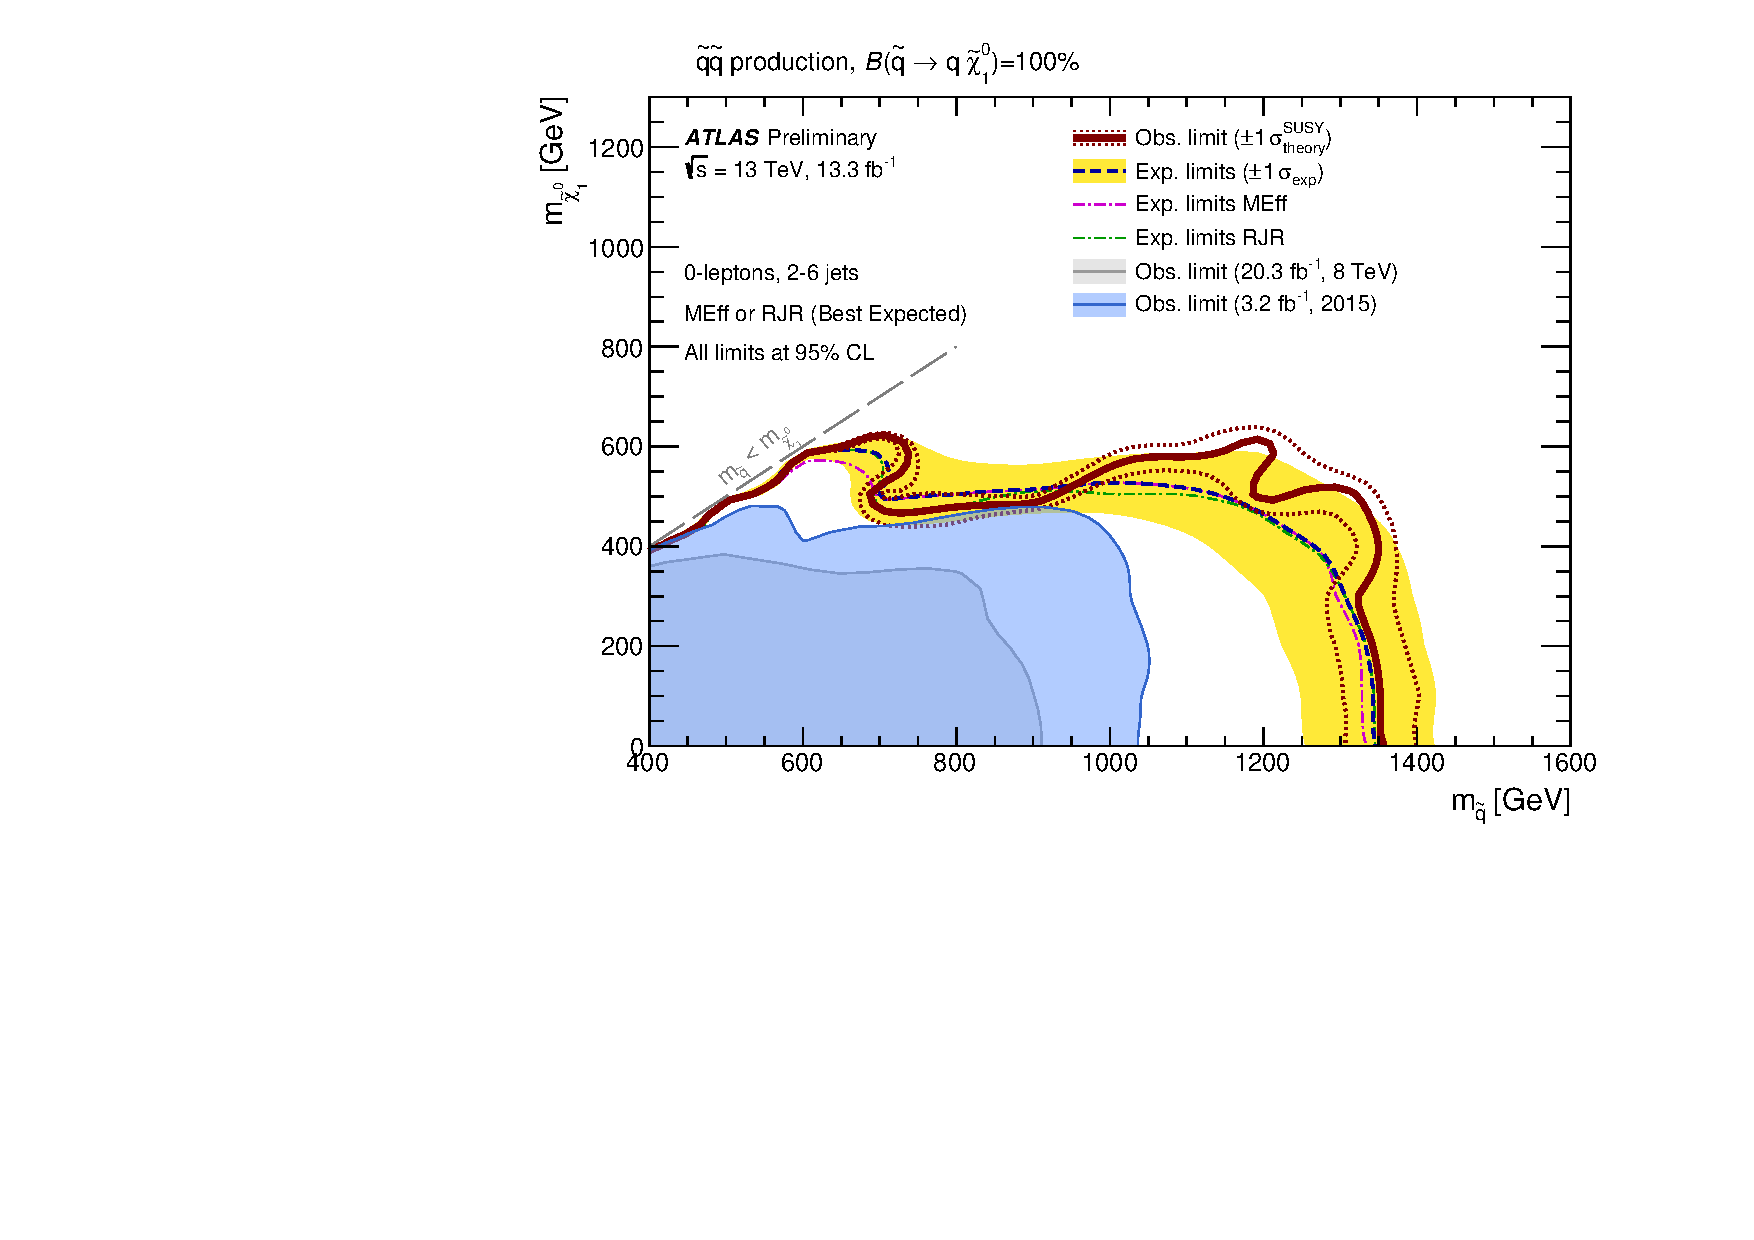
\includegraphics[width=0.49\textwidth]{Farbin/Figures/fig_09a.pdf}}
%% \subfigure{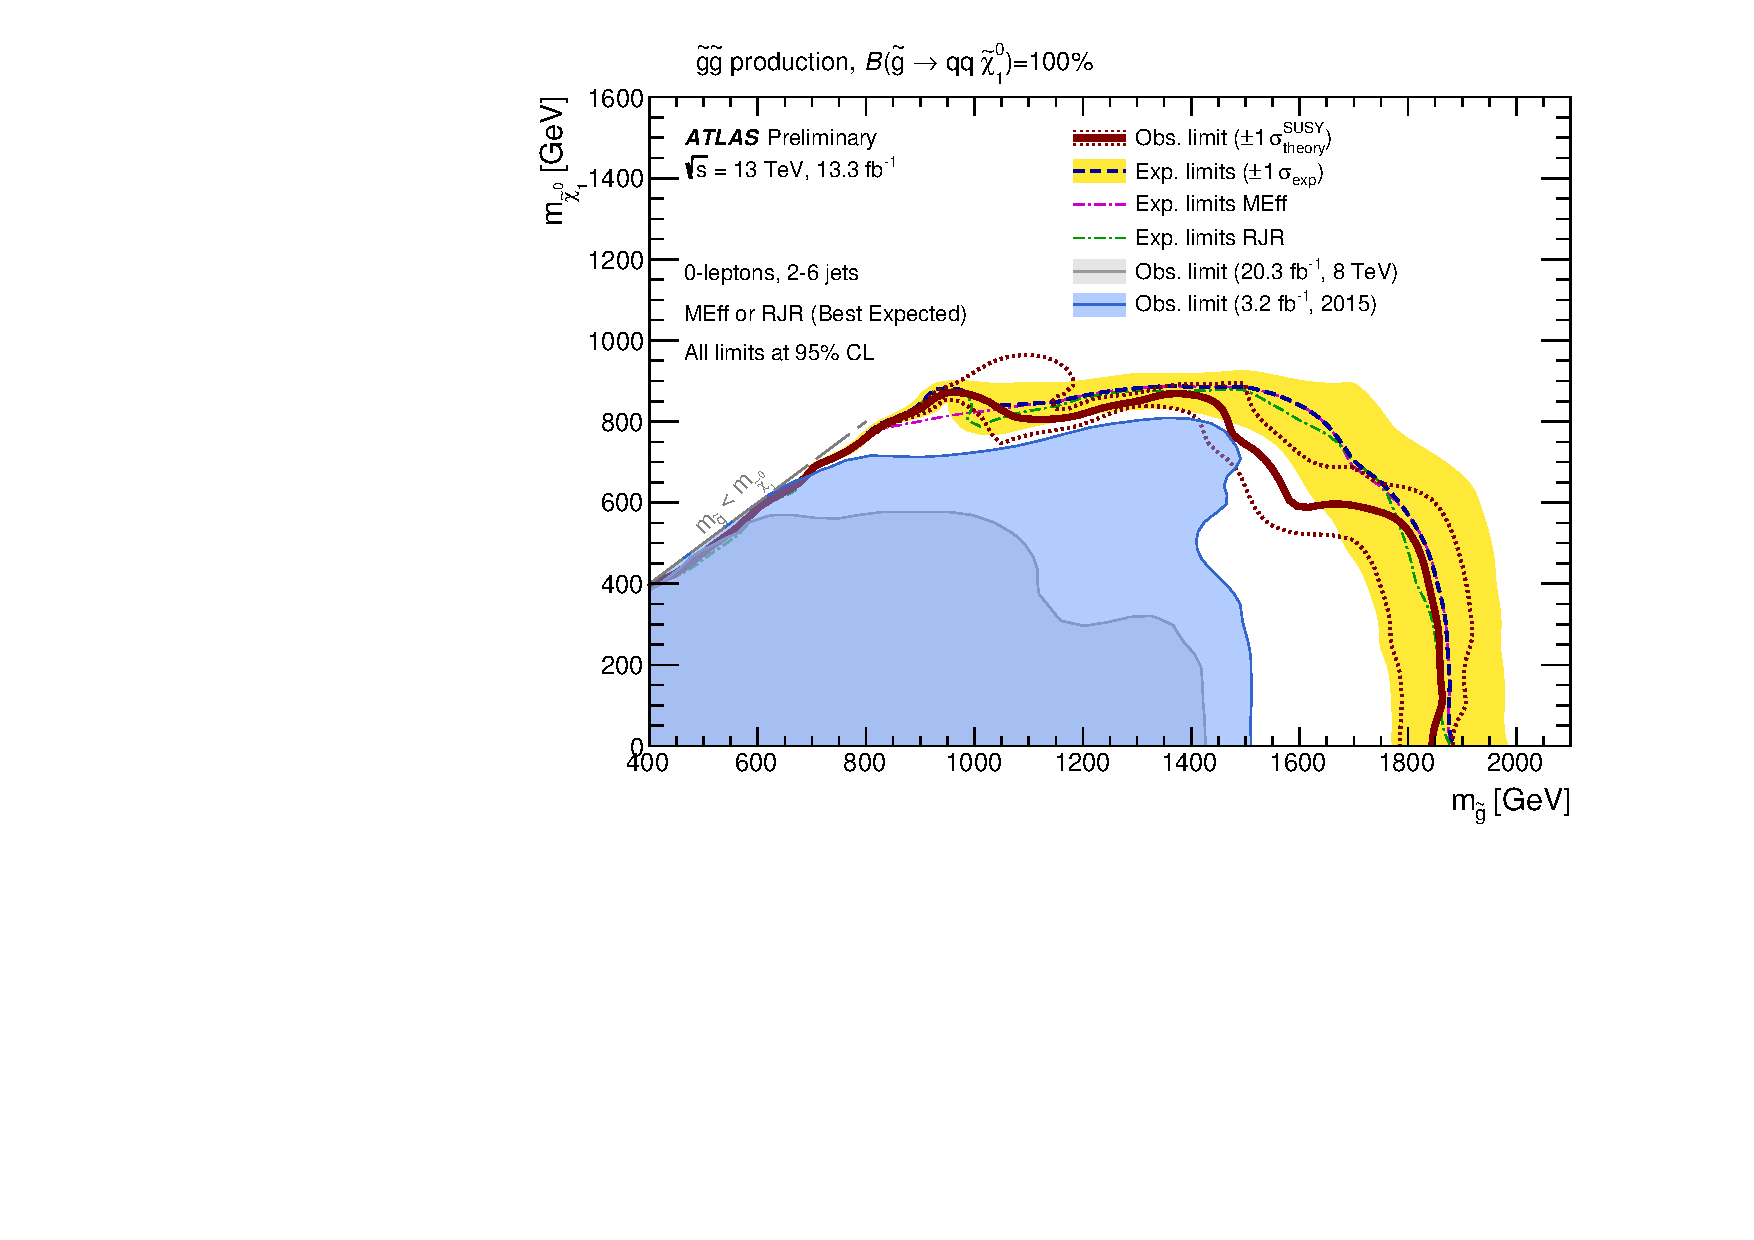
\includegraphics[width=0.49\textwidth]{Farbin/Figures/fig_09b.pdf}}
%% \caption{\label{fig:ICHEPLimits} text
%% }
%% \end{figure}

